% This file is part of the convention of designations for IT inventory.
%
% This convention is a free document: you can redistribute it and/or modify it
% under the terms of the GNU General Public License as published by the Free
% Software Foundation, either version 3 of the License, or (at your option) any
% later version.
%
% This document is distributed in the hope that it will be useful,but WITHOUT
% ANY WARRANTY; without even the implied warranty of MERCHANTABILITY or
% FITNESS FOR A PARTICULAR PURPOSE. See the GNU General Public License for
% more details.
%
% You should have received a copy of the GNU General Public License along with
% this document. If not, see
%
%   http://www.gnu.org/licenses/
%
%
% Copyright (C)
%   2014 Alexander Haase IT Services <support@alexhaase.de>
%

\documentclass[a4paper,11pt]{article}

%
% includes
%
\usepackage{geometry}
\usepackage[utf8]{inputenc}
\usepackage{hyperref}
\usepackage{cite}
\usepackage{amsmath}
\usepackage{float}
\usepackage{multicol}
\usepackage[bottom]{footmisc}
\usepackage{gitinfo}
\usepackage{fancyvrb}
\usepackage{wrapfig}
\usepackage{graphicx}



%
% document style
%
\geometry{a4paper, tmargin=20mm, bmargin=20mm, lmargin=20mm, rmargin=20mm}
\setlength{\parindent}{0pt}

% style for figures
\floatstyle{boxed}
\restylefloat{figure}

% space between two columns
\setlength{\columnsep}{50pt}



%
% document information
%
\title{
	Convention for designations of IT components \\
	\small Version: \gitVtag-\gitAbbrevHash
}
\author{Alexander Haase (\href{mailto:ahaase@alexhaase.de}{ahaase@alexhaase.de})}
\date{\gitAuthorDate}



%
% document
%
\begin{document}
	\maketitle

%	\tableofcontents

	% This file is part of the convention of designations for IT inventory.
%
% This convention is a free document: you can redistribute it and/or modify it
% under the terms of the GNU General Public License as published by the Free
% Software Foundation, either version 3 of the License, or (at your option) any
% later version.
%
% This document is distributed in the hope that it will be useful,but WITHOUT
% ANY WARRANTY; without even the implied warranty of MERCHANTABILITY or
% FITNESS FOR A PARTICULAR PURPOSE. See the GNU General Public License for
% more details.
%
% You should have received a copy of the GNU General Public License along with
% this document. If not, see
%
%   http://www.gnu.org/licenses/
%
%
% Copyright (C)
%   2013-2014 Alexander Haase IT Services <support@alexhaase.de>
%

\section{License}

This convention is a free document: you can redistribute it and/or modify it
under the terms of the GNU General Public License as published by the Free
Software Foundation, either version 3 of the License, or (at your option) any
later version. \\

This document is distributed in the hope that it will be useful, but
\textit{\textbf{without any warranty}}; without even the implied warranty of
\textit{\textbf{merchantability}} or
\textit{\textbf{fitness for a particular purpose}}. See the GNU General Public
License\footnote{\url{http://www.gnu.org/licenses/gpl-3.0}} for more details. \\



\subsection{Copyright}

Copyright \copyright{}   2014 Alexander Haase IT Services
	(\href{mailto:support@alexhaase.de}{support@alexhaase.de})


	% This file is part of the convention of designations for IT inventory.
%
% This convention is a free document: you can redistribute it and/or modify it
% under the terms of the GNU General Public License as published by the Free
% Software Foundation, either version 3 of the License, or (at your option) any
% later version.
%
% This document is distributed in the hope that it will be useful,but WITHOUT
% ANY WARRANTY; without even the implied warranty of MERCHANTABILITY or
% FITNESS FOR A PARTICULAR PURPOSE. See the GNU General Public License for
% more details.
%
% You should have received a copy of the GNU General Public License along with
% this document. If not, see
%
%   http://www.gnu.org/licenses/
%
%
% Copyright (C)
%   2014 Alexander Haase IT Services <support@alexhaase.de>
%

\section{Introduction}

This convention is intended to provide a uniform standard by which all IT
components should be designated. By fixed rules known issues particular to
identify and communication exchange terms are to be avoided.

	% This file is part of the convention of designations for IT inventory.
%
% This convention is a free document: you can redistribute it and/or modify it
% under the terms of the GNU General Public License as published by the Free
% Software Foundation, either version 3 of the License, or (at your option) any
% later version.
%
% This document is distributed in the hope that it will be useful,but WITHOUT
% ANY WARRANTY; without even the implied warranty of MERCHANTABILITY or
% FITNESS FOR A PARTICULAR PURPOSE. See the GNU General Public License for
% more details.
%
% You should have received a copy of the GNU General Public License along with
% this document. If not, see
%
%   http://www.gnu.org/licenses/
%
%
% Copyright (C)
%   2014 Alexander Haase IT Services <support@alexhaase.de>
%

\section{Requirements}

\begin{itemize}
	\item Every designation has to be unique, otherwise two items could be
		confused.

	\item For maintenance and customer support, the designation should be
		clearly stated and read. The case of the letters should be ignored,
		otherwise it is very complicated to spell. Special characters should be
		avoided.

	\item The designation should not be kept short, but not too short, so that
		it could be confused with other numbers.

	\item The designation should contain a few characters to associate a device
		with the designation (e.g. a printer could have pr12345 as designation).
\end{itemize}

	% This file is part of the convention of designations for IT inventory.
%
% This convention is a free document: you can redistribute it and/or modify it
% under the terms of the GNU General Public License as published by the Free
% Software Foundation, either version 3 of the License, or (at your option) any
% later version.
%
% This document is distributed in the hope that it will be useful,but WITHOUT
% ANY WARRANTY; without even the implied warranty of MERCHANTABILITY or
% FITNESS FOR A PARTICULAR PURPOSE. See the GNU General Public License for
% more details.
%
% You should have received a copy of the GNU General Public License along with
% this document. If not, see
%
%   http://www.gnu.org/licenses/
%
%
% Copyright (C)
%   2014 Alexander Haase IT Services <support@alexhaase.de>
%

\section{Charset}

In this convention an derived alphabet of the ``Extended Hex'' Base 32 Alphabet
in RFC 4648 \cite{RFC-4648} will be used. In addition to the described alphabet,
the following characters are \textbf{not} allowed:

\begin{itemize}
	\itemsep 0pt

	\item ``I'' and ``O'' may be confused with ``1'' and ``0''
	\item ``V'' may be confused with ``u'' and ``r''\footnote{\label{foot:handwriting}especially in handwriting}
	\item ``Z'' may be confused with ``2''\footref{foot:handwriting}
\end{itemize}

Instead of forbidding ``0'', ``1'' and ``2'' as recommended in z-base-32
\cite{z-base-32}, all digits are allowed to allow integer-only designations.
For separation ``-'' is also allowed.


\begin{figure}[H]
	\label{fig:charset}

	\begin{verbatim}
		Value Encoding  Value Encoding  Value Encoding  Value Encoding  Value Encoding
		    0 0             7 7            14 E            21 M            28 U
		    1 1             8 8            15 F            22 N            29 W
		    2 2             9 9            16 G            23 P            30 X
		    3 3            10 A            17 H            24 Q            31 Y
		    4 4            11 B            18 J            25 R            32 -
		    5 5            12 C            19 K            26 S
		    6 6            13 D            20 L            27 T
	\end{verbatim}

	\caption{The allowed Alphabet and their representive integer values}
\end{figure}


Any printed label has to be printed in capital letters. In software applications
lowercase letters may be used, but it is recommended to print any information
that is accessable for customers also in \underline{big} capital letters, so
that the designation is clearly readable by them. \\

Software applications that should handle any designation case insensitive, so
the data input is easier for the user.

	% This file is part of the convention of designations for IT inventory.
%
% This convention is a free document: you can redistribute it and/or modify it
% under the terms of the GNU General Public License as published by the Free
% Software Foundation, either version 3 of the License, or (at your option) any
% later version.
%
% This document is distributed in the hope that it will be useful,but WITHOUT
% ANY WARRANTY; without even the implied warranty of MERCHANTABILITY or
% FITNESS FOR A PARTICULAR PURPOSE. See the GNU General Public License for
% more details.
%
% You should have received a copy of the GNU General Public License along with
% this document. If not, see
%
%   http://www.gnu.org/licenses/
%
%
% Copyright (C)
%   2014 Alexander Haase IT Services <support@alexhaase.de>
%

\section{Checksum}
\label{chap:checksum}

To avoid errors when transferring the designation, a check digit is appended to
each designation. \\

The checksum is computed like the check digit of a GTIN\footnote{Global Trade
Item Number} \cite{ean_checksum}. It results from
the modulo 32 (allowed charset without ``-'') of the summed from behind
representive integer value of each character\footnote{\label{foot:charset}see
chapter \ref{fig:charset}}, which are alternately multiplied by weight of 3 and
1. \\

The resulting checksum will be encoded back to its representive
character\footref{foot:charset}.

\begin{minipage}[t]{.45\textwidth}
	\begin{figure}[H]
		\centering

		\begin{tabular}{r|c|c|c|c|c|c}
			i          & 1  & 2  & 3 & 4 & 5 & 6 \\
			\hline
			$x_i$      & A  & B  & 1 & 2 & 3 & 4 \\
			weight     & 1  & 3  & 1 & 3 & 1 & 3 \\
			\hline
			$result_i$ & 10 & 33 & 1 & 6 & 3 & 12 \\
		\end{tabular}

		\begin{align*}
			\sum_{i=0}^{n} result[i] &= 65 \\
			65 \mod 32 &= 1
		\end{align*}

		Complete designation: ``AB12341''.

		\caption{Example for even $n$}
	\end{figure}
\end{minipage}
\hfill
\begin{minipage}[t]{.45\textwidth}
	\begin{figure}[H]
		\centering

		\begin{tabular}{r|c|c|c|c|c|c|c}
			i          & 1  & 2  & 3 & 4 & 5 & 6 & 7 \\
			\hline
			$x_i$      & A  & B  & 1 & 2 & 3 & 4 & 5 \\
			weight     & 3  & 1  & 3 & 1 & 3 & 1 & 3 \\
			\hline
			$result_i$ & 30 & 11 & 3 & 2 & 9 & 4 & 15 \\
		\end{tabular}

		\begin{align*}
			\sum_{i=0}^{n} result[i] &= 74 \\
			74 \mod 32 &= 10 \hat{=} A
		\end{align*}

		Complete designation: ``AB12345A''.

		\caption{Example for odd $n$}
	\end{figure}
\end{minipage} \\


This algorithm could be written as mathematical function for the string $x$ with
length $n$:
\begin{align*}
	f(x, n) &= \sum_{i=0}^{n-1} x_i \left( 1 + 2 \left( \left( n - i \right) mod
		2 \right) \right) \mod 32
\end{align*}

	% This file is part of the convention of designations for IT inventory.
%
% This convention is a free document: you can redistribute it and/or modify it
% under the terms of the GNU General Public License as published by the Free
% Software Foundation, either version 3 of the License, or (at your option) any
% later version.
%
% This document is distributed in the hope that it will be useful,but WITHOUT
% ANY WARRANTY; without even the implied warranty of MERCHANTABILITY or
% FITNESS FOR A PARTICULAR PURPOSE. See the GNU General Public License for
% more details.
%
% You should have received a copy of the GNU General Public License along with
% this document. If not, see
%
%   http://www.gnu.org/licenses/
%
%
% Copyright (C)
%   2014 Alexander Haase IT Services <support@alexhaase.de>
%

\section{Specification}

\textit{All designations are constructed according to the following pattern, if
not otherwise specified in the relevant specification.} \\


A designation starts with an one to three alphanumerical ``device identifier''
followed by a alphanumeric ``ID string'' and terminated by the checksum as
defined in chapter \ref{chap:checksum}. The ``device identifier''
\underline{must} begin with letters and may be continued with a number. If
numbers are used in the ``device identifier'', a hypen must seperate the
``device identifier'' and ``ID string''. \\

The maximum length of the whole designation \underline{without hyphens} is 10. A
group of characters between hyphens may not be longer than 4 characters.



%
% include specific conventions
%

% This file is part of the convention of designations for IT inventory.
%
% This convention is a free document: you can redistribute it and/or modify it
% under the terms of the GNU General Public License as published by the Free
% Software Foundation, either version 3 of the License, or (at your option) any
% later version.
%
% This document is distributed in the hope that it will be useful,but WITHOUT
% ANY WARRANTY; without even the implied warranty of MERCHANTABILITY or
% FITNESS FOR A PARTICULAR PURPOSE. See the GNU General Public License for
% more details.
%
% You should have received a copy of the GNU General Public License along with
% this document. If not, see
%
%   http://www.gnu.org/licenses/
%
%
% Copyright (C)
%   2014 Alexander Haase IT Services <support@alexhaase.de>
%

\subsection{Device Identifier}
\label{chap:con_dev-identify}


\subsubsection{Network infrastructure}

\begin{tabular}{p{1.4cm}p{15cm}}
	APL	& $UK_0$ port of the telecommuncation provider. ``ID string'' is an
		integer representing the TAE/APL port number. (e.g. TAE1/APL1 would be
		``APL16''). This designation should only be used in documentations, but
		the normal network port designation (see chapter \ref{chap:con_netport})
		should be used.
\end{tabular}



\subsubsection{Computer / server / virtual machines}

\begin{tabular}{p{1.4cm}p{15cm}}
	SRV	& Server \\

	WST	& Workstation and standalone computer \\

	VC	& Virtual container \\

	VM	& Virtual machine \\
\end{tabular}



\subsubsection{Printers and similar hardware}

\begin{tabular}{p{1.4cm}p{15cm}}
	PR	& common printer (laser and inkjet) with or without multifunction (e.g.
		scanner or fax) \\

	SC	& standalone scanner \\

	FAX	& standalone fax and fax gateways \\
\end{tabular}

% This file is part of the convention of designations for IT inventory.
%
% This convention is a free document: you can redistribute it and/or modify it
% under the terms of the GNU General Public License as published by the Free
% Software Foundation, either version 3 of the License, or (at your option) any
% later version.
%
% This document is distributed in the hope that it will be useful,but WITHOUT
% ANY WARRANTY; without even the implied warranty of MERCHANTABILITY or
% FITNESS FOR A PARTICULAR PURPOSE. See the GNU General Public License for
% more details.
%
% You should have received a copy of the GNU General Public License along with
% this document. If not, see
%
%   http://www.gnu.org/licenses/
%
%
% Copyright (C)
%   2014 Alexander Haase IT Services <support@alexhaase.de>
%

\subsection{Provider connections}
\label{chap:spec_provider_conn}

The ``APL'' designations depend on designations of your telecommunication
provider. Regular your provider will tell you, at which ``APL'' port a givven
number is connected. You may need this number, if you have to connect new wires
to the APL-port, so it will be usefull to write this number down. \\

The ``TAE'' designation depends on the ``APL'' designation: If the wire is
connected to APL-port 9, then it will be ``TAE9''. \\

\textbf{Note:} \textit{For ``APL'' and ``TAE'' designations, no
checksum\footnote{\label{foot:checksum}see chapter \ref{chap:checksum}} will be
appended, otherwise there could be problems when you want to reference these by
the telecommunication provider.}

% This file is part of the convention of designations for IT inventory.
%
% This convention is a free document: you can redistribute it and/or modify it
% under the terms of the GNU General Public License as published by the Free
% Software Foundation, either version 3 of the License, or (at your option) any
% later version.
%
% This document is distributed in the hope that it will be useful,but WITHOUT
% ANY WARRANTY; without even the implied warranty of MERCHANTABILITY or
% FITNESS FOR A PARTICULAR PURPOSE. See the GNU General Public License for
% more details.
%
% You should have received a copy of the GNU General Public License along with
% this document. If not, see
%
%   http://www.gnu.org/licenses/
%
%
% Copyright (C)
%   2014 Alexander Haase IT Services <support@alexhaase.de>
%

\subsection{Network Ports}
\label{chap:spec_netport}

\begin{wrapfigure}{r}{0.35\textwidth}
	Room: 212; Port: 6 \\
	Basic designation: ESC-212-6 \\

	Caclulation of the checksum:
	\begin{align*}
		\sum_{i=0}^{n} x_i &= 192 \\
		192 \mod 32 &= 7
	\end{align*}

	The complete designation will be ``ESC-212-67''.

	\caption{Example network port designation for ethernet}
\end{wrapfigure}

A designation for a network port consists of the device identifier, a room and a
port number seperated by dash ``-'' and a checksum\footref{foot:checksum}. \\

The designation should be written at the top of the network port. If the
network port has two RJ45-plugs, two letters seperated by slash will be
appended. Regular these will be ``A/B'', but if two network ports will be side
by side, they may share the port-number, but the letters will change to e.g.
``C/D''. The first letter wll always be the left plug, the second the right. For
fiber ports (or network ports that are turned $90^{\circ}$) the first will
always be top and the second the bottom. \\

The letters belong to the name of one of the two network ports (e.g. the
name of the left network port could be ``ESC-212-67A''), but they are
\underline{not} considered in the calculation of the checksum. \\


\begin{minipage}[t]{.42\textwidth}
	\begin{figure}[H]
		\begin{verbatim}

			      ########################
			      #                      #
			      #      212-67 A/B      #
			      #                      #
			      #   ######    ######   #
			      #   #    #    #    #   #
			      #   #    #    #    #   #
			      #   ######    ######   #
			      #                      #
			      #                      #
			      ########################
		\end{verbatim}

		\caption{Example network port labeling (normal)}
	\end{figure}
\end{minipage}
\hfill
\begin{minipage}[t]{.42\textwidth}
	\begin{figure}[H]
		\begin{verbatim}

			       #######################
			       #                     #
			       #      212-67 A/B     #
			       #                     #
			       #      ##########     #
			       #      ##########     #
			       #                     #
			       #      ##########     #
			       #      ##########     #
			       #                     #
			       #######################
		\end{verbatim}

		\caption{Example network port labeling (vertical)}
	\end{figure}
\end{minipage} \\

For ethernet cabeling, the device identifier will be ``ESC'', for ISDN ``ISC''.
It is irrelevant, if the singal is ethernet or ISDN, but it will be ``ISC'', if
not eight but only four wires are connected to the network-port. This implifies,
that a ISDN device may also be connected to an ESC-port, if it is switched to
an NTBA. \\

For ethernet network ports, the device identifier does not need to be printed
on an human readable label, but must be included in any digital label that is
proccessed non-human (e.g. QR code or databases).


	% This file is part of the convention of designations for IT inventory.
%
% This convention is a free document: you can redistribute it and/or modify it
% under the terms of the GNU General Public License as published by the Free
% Software Foundation, either version 3 of the License, or (at your option) any
% later version.
%
% This document is distributed in the hope that it will be useful,but WITHOUT
% ANY WARRANTY; without even the implied warranty of MERCHANTABILITY or
% FITNESS FOR A PARTICULAR PURPOSE. See the GNU General Public License for
% more details.
%
% You should have received a copy of the GNU General Public License along with
% this document. If not, see
%
%   http://www.gnu.org/licenses/
%
%
% Copyright (C)
%   2014 Alexander Haase IT Services <support@alexhaase.de>
%

\section{QR codes}

\begin{wrapfigure}{r}{0.25\textwidth}
	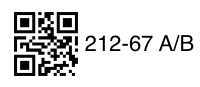
\includegraphics[width=0.2\textwidth]{qr.png}

	\caption{Example network port designation}
\end{wrapfigure}

For better maintenance a QR code could be added to designation labels, so the
customer or maintenance stuff is able to scan the information instead of typing
it in the device. It is recommended, to print it a little bit bigger than
required, so that it is still scanable unter bad conditions. \\

\textbf{Note:} The QR code should contain the \underline{full} designation
includuding the designation identifier.



	% add references
	\nocite{*}
	\bibliography{references}{}
	\bibliographystyle{plain}
\end{document}
